\section{Problem Background}
In large-scale data intensive problems with geographically distributed resources,  load is generated from multiple sources\cite{moges2009grid} for a class of problems.  It is assumed that the problem representation can be divided amongst the processors.  Thus the problem representation is said to be ``divisible".  The processing of massive amounts of data on distributed and parallel networks is becoming more and more common.  The problem of minimizing the processing time of extensive loads originating from a multiplicity of sources and being processed on a multiplicity of nodes presents a challenge.  \\
In this chapter, the closed-form processor equivalence\cite{robertazzi1993processor}\cite{Liu_1schedulingdivisible} problem in the grid network of regular network and toroidal rectangle network is discussed.  Also, the multi-source workload assignment is also taken into account.

In this thesis, we investigate two problems. One is the processor equivalence.  The other one is scheduling divisible workloads from multiple sources in regular network \Fig{5t5}, toroidal rectangle network \Fig{torusnetwork} and hypercube network \Fig{hypercube}.\\

\begin{figure}[!ht]
\centering
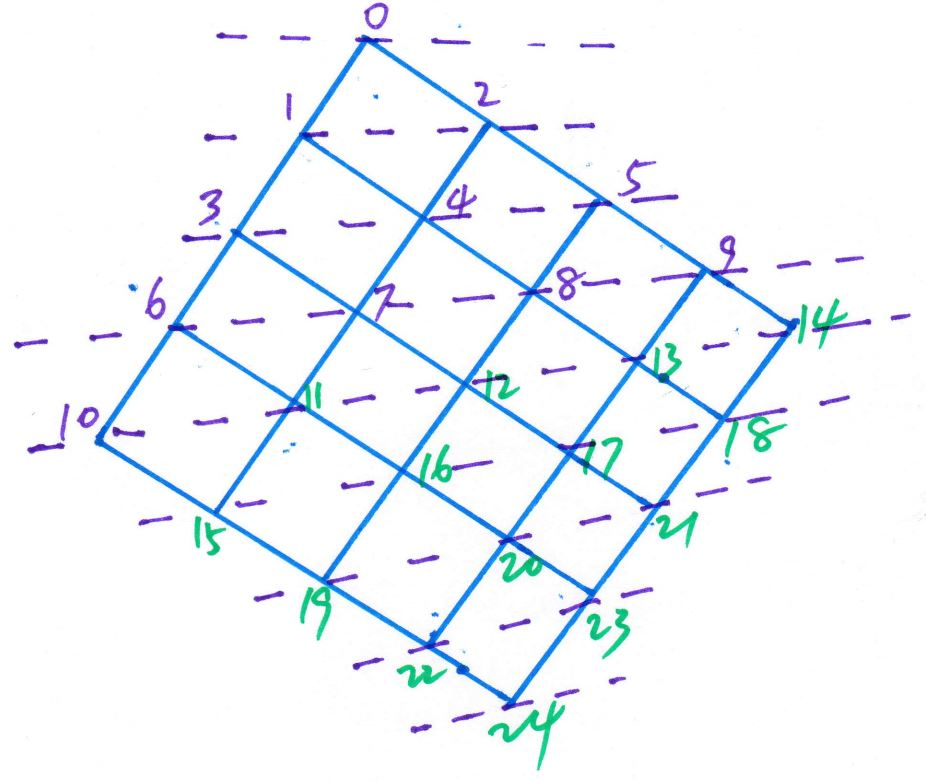
\includegraphics[width=0.8\columnwidth]{figure/5t5.JPG}
\caption{A m*n regular network(m = 5,  n = 5)}
\label{fig:5t5}
\end{figure}

\begin{figure}[!ht]
\centering
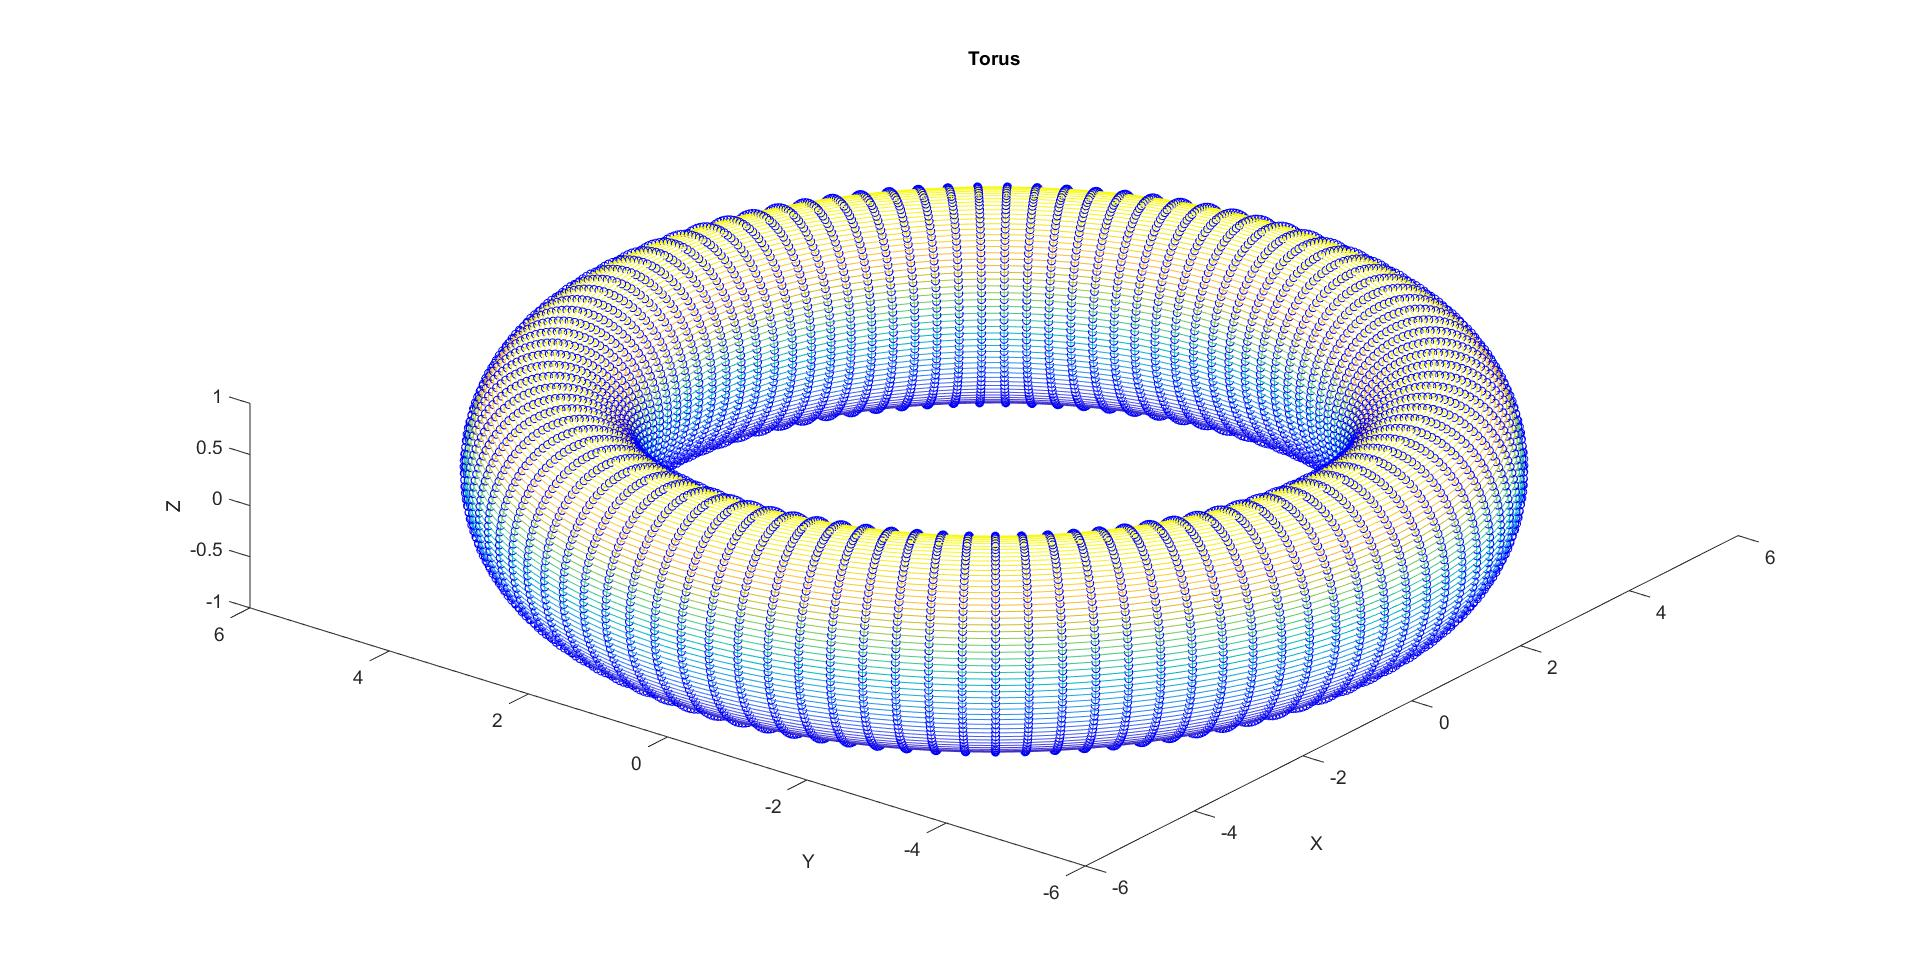
\includegraphics[width=1\columnwidth]{figure/torusnetwork.jpg}
\caption{A toroidal rectangle network with grid unit cores}
\label{fig:torusnetwork}
\end{figure}

\begin{figure}[!ht]
\centering
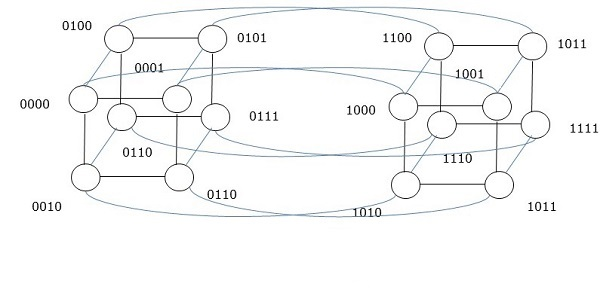
\includegraphics[width=0.8\columnwidth]{figure/hypercube.jpg}
\caption{A hypercube network}
\label{fig:hypercube}
\end{figure}
\newpage 

\section{Definitions and Assumption}

\theoremstyle{definition}
\begin{definition}{Equal Computation}\\
Equal computation is a technique, which considers combining a cluster of processors as one whole processor to process the unit $1$ workload.
\end{definition}

The following assumptions are used throughout the paper:

\begin{itemize}
\item The virtual cut through \cite{kermani1979virtual} switching is used to transmit the assigned workload between processors.
\item For simply, we do not consider return communications.  
\item The communication delays are taken into consideration.  
\item The time costs of computation and communication are assumed to be linear function of the data size.  
\item The network environment is homogeneous, that is, all the processors have the same computation capacity.  The link speeds between any two unit cores are identical.   
\item The number of outgoing ports in each processor is limited.  In NOC(network on chip), the port number is fixed 4 or 5.  
\item The general graph's grid node's in-degree and out-degree is 4 or 5.  
\end{itemize}

The optimization objective functions are as follows :
\begin{itemize}
\item Equal computation : the problem's objective function is how to partition and schedule the workloads amongst the processors to get the minimum finish time.  
\item Multi-source assignment : how to finish the unit $1$ workload at the same time utilizing smaller processor.
\end{itemize}

To achieve the minimum solution is obtained by forcing the processors over a network to stop processing simultaneously.  Intuitively, this is because the solution could be improved by transfer load from some busy processor to idle ones.  

\subsection{Notions}
The following notations and definitions are utilized:
\begin{itemize}
\item $P_{i}$: The $i$th processor.   $0  \leq i \leq m*n-1$.  
\item $L_{i}$: The $i$th work load.   $1 \leq i \leq k$.  
\item $D_{i}$: The minimum number of hops from the processor $P_{i}$ to the data load injection $L$.  
\item $level_{i}$: The processors have $i$ minimum Manhattan distance to the data injection.
\item $\alpha_{0}$: The load fraction assigned to the root processor.  
\item $\alpha_{i}$: The load fraction assigned to the $i$th processor.  
\item $\omega_{i}$: The inverse computing speed on the $i$th processor.  
\item $\omega_{eq}$: The inverse computing speed on an equivalent node collapsed from a cluster of processors.  

\item $z_{i}$: The inverse link speed on the $i$th link.  
\item $T_{cp}$: Computing intensity constant.  The entire load is processed in $\omega_{i}T_{cp}$ on the $i$th processor.  

\item $T_{cm}$: Communication intensity constant.  The entire load is transmitted in $z_{i}T_{cm}$ seconds over the $i$th link.  
\item $T_{f, n}$: The finish time of the whole processor network.  Here $T_{f, n}$ is equal to $\omega_{eq}T_{cp}$.  

\item $T_{f, 0}$: The finish time for the entire divisible load solved on the root processor.  Here $T_{f, 0}$ is equal to $1 \times \omega_{0}T_{cp}$,  that is $\omega_{0}T_{cp}$.  

\item $\sigma = \frac{zT_{cm}}{\omega T_{cp}}$: The ratio between the communication speed to the computation speed,  $0 < \sigma < 1$ \cite{bharadwaj1996scheduling} \cite{hung2004switching}.  

\item In multi-source situation, $\sum_{i = 1}^{k} L_{i} = 1$
\item $\sum_{i = 0}^{m*n-1} \alpha_{i}= 1$
\item $Speedup = \frac{T_{f, 0}}{T_{f, n}}= \frac{\omega T_{cp}}{\alpha_{0}\omega T_{cp}} = \frac{1}{\alpha_{0}}$
\end{itemize}
\newpage